\chapter*{Appendices}
\section*{Uncertainties}
The uncertainties used for gravametric calculation of gas standard is the quadrature sum of the weighing uncertainties before and after the transfer of the component into the vessel.
\begin{table}[H]
    \centering
    \begin{tabular}{@{}cc@{}}
    \toprule
    Balance                   & Standard uncertainty \\ \midrule
    Mettler Toledo XPE26003LC & 20.0 mg                \\
    Satorius 1475 MP8         & 1.4 mg               \\
    Mettler Toledo PR2004     & 0.3 mg               \\
    Mettler Toledo XP2004S    & 0.3 mg               \\
    Mettler Toledo XP205      & 0.1 mg               \\
    Sartorius R160P           & 0.1 mg               \\ \bottomrule
    \end{tabular}
    \caption*{Standard uncertainties (k=1) of the balances used for gravametric preparation of gas standards}
\end{table}
\section*{Simulation files}
\subsection*{Hydrogen impurities}
\subsubsection*{Ammonia}
\begin{verbatim}
    &CONTROL
    calculation='relax',
    outdir='./tmp/',
    prefix='Ammonia',
    pseudo_dir='/home/mp916/Simulations/qe/qe-6.1/Simulationpdpaper/Pseudo',
    verbosity='high',
    forc_conv_thr = 0.000583,
    tprnfor = .TRUE.
  /
  
  &SYSTEM
    ibrav=0,
    celldm(1)=15.1474115563d0,
    nat=4,
    ntyp=2,
    ecutwfc=30,
    ecutrho=120,
    occupations='smearing',
    degauss=0.005d0,
  /
  &ELECTRONS
    mixing_ndim = 20
    mixing_beta = 0.8
    conv_thr=1d-05,
  /
  &IONS
  /
  ATOMIC_SPECIES
    H 1.007940d0 H.pw91-kjpaw_psl.1.0.0.UPF
    N 14.006700d0 N.pw91-n-kjpaw_psl.1.0.0.UPF
  ATOMIC_POSITIONS {crystal}
     N   0.5042649612d0   0.4816814914d0   0.5185608552d0
     H   0.5858110338d0   0.5710210191d0   0.4807806443d0
     H   0.4526766026d0   0.4289789809d0   0.4165818655d0
     H   0.4141889662d0   0.5407708619d0   0.5834181345d0
  K_POINTS {automatic}
    8 8 8 0 0 0
  CELL_PARAMETERS {alat}
    1.000000000000d0  0.000000000000d0  0.000000000000d0
    0.000000000000d0  0.968552952250d0  0.000000000000d0
    0.000000000000d0  0.000000000000d0  0.994255872719d0
\end{verbatim}
\subsubsection*{Argon}
\begin{verbatim}
    &CONTROL
    calculation='scf',
    outdir='./tmp/',
    prefix='Ar',
    pseudo_dir='/home/mp916/Simulations/qe/qe-6.1/Simulationpdpaper/Pseudo',
    verbosity='high',
    forc_conv_thr = 0.000583,
    tprnfor = .TRUE.
  /
  
  &SYSTEM
    ibrav=0,
    celldm(1)=15.0422199515d0,
    nat=1,
    ntyp=1,
    ecutwfc=30,
    ecutrho=120,
    occupations='smearing',
    smearing='mv',
    degauss=0.005d0,
  /
  
  &ELECTRONS
    mixing_mode = 'local-TF'
    mixing_ndim = 20
    mixing_beta = 0.3
    conv_thr=1d-05,
  /
  
  ATOMIC_SPECIES
    Ar 39.948000d0 Ar.pw91-nl-kjpaw_psl.1.0.0.UPF
  
  ATOMIC_POSITIONS {crystal}
    Ar   0.5000000000d0   0.5000000000d0   0.5000000000d0
  
  K_POINTS {automatic}
    8 8 8 0 0 0
  
  CELL_PARAMETERS {alat}
    1.000000000000d0  0.000000000000d0  0.000000000000d0
    0.000000000000d0  1.000000000000d0  0.000000000000d0
    0.000000000000d0  0.000000000000d0  1.000000000000d0
  
\end{verbatim}

\subsubsection*{Carbon Dioxide}
\begin{verbatim}
    
&CONTROL
calculation='relax',
outdir='./tmp/',
prefix='CO2',
pseudo_dir='/home/mp916/Simulations/qe/qe-6.1/Simulationpdpaper/Pseudo',
verbosity='high',
forc_conv_thr = 0.000583,
tprnfor = .TRUE.
/

&SYSTEM
ibrav=0,
celldm(1)=15.5625245542d0,
nat=3,
ntyp=2,
ecutwfc=30,
ecutrho=120,
occupations='smearing',
smearing='mv',
degauss=0.005d0,
/

&ELECTRONS
mixing_mode = 'local-TF'
mixing_ndim = 20
mixing_beta = 0.3
conv_thr=1d-05,
/

&IONS

/

ATOMIC_SPECIES
C 12.010700d0 C.pw91-n-kjpaw_psl.1.0.0.UPF
O 15.999400d0 O.pw91-n-kjpaw_psl.1.0.0.UPF

ATOMIC_POSITIONS {crystal}
 C   0.5000000007d0   0.5000000008d0   0.4999999998d0
 O   0.4529264144d0   0.4999999999d0   0.3864094181d0
 O   0.5470735856d0   0.4999999992d0   0.6135905819d0

K_POINTS {automatic}
8 8 8 0 0 0

CELL_PARAMETERS {alat}
1.000000000000d0  0.000000000000d0  0.000000000000d0
0.000000000000d0  0.915567068158d0  0.000000000000d0
0.000000000000d0  0.000000000000d0  1.172141239726d0


\end{verbatim}

\subsubsection*{Carbon Monoxide}
\begin{verbatim}
    
&CONTROL
calculation='relax',
outdir='./tmp/',
prefix='CO',
pseudo_dir='/home/mp916/Simulations/qe/qe-6.1/Simulationpdpaper/Pseudo',
verbosity='high',
forc_conv_thr = 0.000583,
tprnfor = .TRUE.
/

&SYSTEM
ibrav=0,
celldm(1)=14.2485349792d0,
nat=2,
ntyp=2,
ecutwfc=30,
ecutrho=120,
occupations='smearing',
smearing='mv',
degauss=0.005d0,
/

&ELECTRONS
mixing_mode = 'local-TF'
mixing_ndim = 20
mixing_beta = 0.3
conv_thr=1d-05,
/

&IONS

/

ATOMIC_SPECIES
C 12.010700d0 C.pw91-n-kjpaw_psl.1.0.0.UPF
O 15.999400d0 O.pw91-n-kjpaw_psl.1.0.0.UPF

ATOMIC_POSITIONS {crystal}
 O   0.5000270812d0   0.5738644516d0   0.5000000000d0
 C   0.4999729188d0   0.4261355484d0   0.5000000000d0

K_POINTS {automatic}
8 8 8 0 0 0

CELL_PARAMETERS {alat}
1.000000000000d0  0.000000000000d0  0.000000000000d0
0.000000000000d0  1.167110986173d0  0.000000000000d0
0.000000000000d0  0.000000000000d0  1.000000000000d0
\end{verbatim}

\subsubsection*{Formaldehyde}
\begin{verbatim}
    
&CONTROL
calculation='relax',
outdir='./tmp/',
prefix='Formaldehyde',
pseudo_dir='/home/mp916/Simulations/qe/qe-6.1/Simulationpdpaper/Pseudo',
verbosity='high',
forc_conv_thr = 0.000583,
tprnfor = .TRUE.
/

&SYSTEM
ibrav=0,
celldm(1)=14.2485349792d0,
nat=4,
ntyp=3,
ecutwfc=30,
ecutrho=120,
occupations='smearing',
smearing='mv',
degauss=0.005d0,
/

&ELECTRONS
mixing_mode = 'local-TF'
mixing_ndim = 20
mixing_beta = 0.3
conv_thr=1d-05,
/

&IONS

/

ATOMIC_SPECIES
C 12.010700d0 C.pw91-n-kjpaw_psl.1.0.0.UPF
O 15.999400d0 O.pw91-n-kjpaw_psl.1.0.0.UPF
H 1.007940d0 H.pw91-kjpaw_psl.1.0.0.UPF

ATOMIC_POSITIONS {crystal}
 H   0.5000032071d0   0.3993778194d0   0.6091900164d0
 C   0.4999967927d0   0.4644674926d0   0.4999863532d0
 H   0.5000032073d0   0.3993419309d0   0.3908099836d0
 O   0.5000031360d0   0.6006580691d0   0.4999707562d0

K_POINTS {automatic}
8 8 8 0 0 0

CELL_PARAMETERS {alat}
1.000000000000d0  0.000000000000d0  0.000000000000d0
0.000000000000d0  1.170692569629d0  0.000000000000d0
0.000000000000d0  0.000000000000d0  1.126681305036d0


\end{verbatim}

\subsubsection*{Formic acid}
\begin{verbatim}
    
&CONTROL
calculation='relax',
outdir='./tmp/',
prefix='Formicacid',
pseudo_dir='/home/mp916/Simulations/qe/qe-6.1/Simulationpdpaper/Pseudo',
verbosity='high',
forc_conv_thr = 0.000583,
tprnfor = .TRUE.
/

&SYSTEM
ibrav=0,
celldm(1)=17.2803095283d0,
nat=5,
ntyp=3,
ecutwfc=30,
ecutrho=120,
occupations='smearing',
smearing='mv',
degauss=0.005d0,
/

&ELECTRONS
mixing_mode = 'local-TF'
mixing_ndim = 20
mixing_beta = 0.3
conv_thr=1d-05,
/

&IONS

/

ATOMIC_SPECIES
C 12.010700d0 C.pw91-n-kjpaw_psl.1.0.0.UPF
O 15.999400d0 O.pw91-n-kjpaw_psl.1.0.0.UPF
H 1.007940d0 H.pw91-kjpaw_psl.1.0.0.UPF

ATOMIC_POSITIONS {crystal}
 H   0.6145158987d0   0.4838354467d0   0.3823127673d0
 C   0.5065122208d0   0.4904111511d0   0.4330303046d0
 O   0.3854841013d0   0.4782033285d0   0.3808877459d0
 O   0.5145431942d0   0.5163076772d0   0.5762053140d0
 H   0.4199060272d0   0.5217966715d0   0.6191122541d0

K_POINTS {automatic}
8 8 8 0 0 0

CELL_PARAMETERS {alat}
1.000000000000d0  0.000000000000d0  0.000000000000d0
0.000000000000d0  0.848121779294d0  0.000000000000d0
0.000000000000d0  0.000000000000d0  1.013821874194d0


\end{verbatim}

\subsubsection*{Hydrogen}
\begin{verbatim}
    
&CONTROL
calculation='relax',
outdir='./tmp/',
prefix='Hydrogen',
pseudo_dir='/home/mp916/Simulations/qe/qe-6.1/Simulationpdpaper/Pseudo',
verbosity='high',
forc_conv_thr = 0.000583,
tprnfor = .TRUE.
/

&SYSTEM
ibrav=0,
celldm(1)=12.6119438239d0,
nat=2,
ntyp=1,
ecutwfc=30,
ecutrho=120,
occupations='smearing',
smearing='mv',
degauss=0.005d0,
/

&ELECTRONS
mixing_mode = 'local-TF'
mixing_ndim = 20
mixing_beta = 0.3
conv_thr=1d-05,
/

&IONS


/

ATOMIC_SPECIES
H 1.007940d0 H.pw91-kjpaw_psl.1.0.0.UPF

ATOMIC_POSITIONS {crystal}
 H   0.5025437140d0   0.5504756643d0   0.4980656210d0
 H   0.4974562860d0   0.4495243357d0   0.5019343790d0

K_POINTS {automatic}
8 8 8 0 0 0

CELL_PARAMETERS {alat}
1.000000000000d0  0.000000000000d0  0.000000000000d0
-0.500000000000d0  0.866025403784d0  0.000000000000d0
0.000000000000d0  0.000000000000d0  3.858856497911d0
\end{verbatim}

\subsubsection*{Helium}
\begin{verbatim}
    
&CONTROL
calculation='scf',
outdir='./tmp/',
prefix='He',
pseudo_dir='/home/mp916/Simulations/qe/qe-6.1/Simulationpdpaper/Pseudo',
verbosity='high',
forc_conv_thr = 0.000583,
tprnfor = .TRUE.
/

&SYSTEM
ibrav=0,
celldm(1)=14.8532473391d0,
nat=1,
ntyp=1,
ecutwfc=30,
ecutrho=120,
occupations='smearing',
smearing='mv',
degauss=0.005d0,
/

&ELECTRONS
mixing_mode = 'local-TF'
mixing_ndim = 20
mixing_beta = 0.3
conv_thr=1d-05,
/

&IONS

/

ATOMIC_SPECIES
He 4.002600d0 He.pw91-kjpaw_psl.1.0.0.UPF

ATOMIC_POSITIONS {crystal}
He   0.5000000000d0   0.5000000000d0   0.5000000000d0

K_POINTS {automatic}
8 8 8 0 0 0

CELL_PARAMETERS {alat}
1.000000000000d0  0.000000000000d0  0.000000000000d0
0.000000000000d0  1.000000000000d0  0.000000000000d0
0.000000000000d0  0.000000000000d0  1.000000000000d0


\end{verbatim}

\subsubsection*{Hydrogen Sulphide}
\begin{verbatim}
    
&CONTROL
calculation='relax',
outdir='./tmp/',
prefix='h2s',
pseudo_dir='/home/mp916/Simulations/qe/qe-6.1/Simulationpdpaper/Pseudo',
verbosity='high',
forc_conv_thr = 0.000583,
tprnfor = .TRUE.
/

&SYSTEM
ibrav=0,
celldm(1)=16.0398870722d0,
nat=3,
ntyp=2,
ecutwfc=30,
ecutrho=120,
occupations='smearing',
smearing='mv',
degauss=0.005d0,
/

&ELECTRONS
mixing_mode = 'local-TF'
mixing_ndim = 20
mixing_beta = 0.3
conv_thr=1d-05,
/

&IONS

/

ATOMIC_SPECIES
H 1.007940d0 H.pw91-kjpaw_psl.1.0.0.UPF
S 32.065000d0 S.pw91-nl-kjpaw_psl.1.0.0.UPF

ATOMIC_POSITIONS {crystal}
 H   0.5676219636d0   0.4950645124d0   0.3911640247d0
 S   0.4323780364d0   0.5049354876d0   0.4708913462d0
 H   0.5069112201d0   0.4960181453d0   0.6088359753d0

K_POINTS {automatic}
8 8 8 0 0 0

CELL_PARAMETERS {alat}
1.000000000000d0  0.000000000000d0  0.000000000000d0
0.000000000000d0  0.947225998108d0  0.000000000000d0
0.000000000000d0  0.000000000000d0  1.003132863700d0


\end{verbatim}

\subsubsection*{Methane}
\begin{verbatim}
    
&CONTROL
calculation='relax',
outdir='./tmp/',
prefix='ch4',
pseudo_dir='/home/mp916/Simulations/qe/qe-6.1/Simulationpdpaper/Pseudo',
verbosity='high',
forc_conv_thr = 0.000583,
tprnfor = .TRUE.
/

&SYSTEM
ibrav=0,
celldm(1)=15.5988312226d0,
nat=5,
ntyp=2,
ecutwfc=30,
ecutrho=120,
occupations='smearing',
smearing='mv',
degauss=0.005d0,
/

&ELECTRONS
mixing_mode = 'local-TF'
mixing_ndim = 20
mixing_beta = 0.3
conv_thr=1d-05,
/

&IONS

/

ATOMIC_SPECIES
C 12.010700d0 C.pw91-n-kjpaw_psl.1.0.0.UPF
H 1.007940d0 H.pw91-kjpaw_psl.1.0.0.UPF

ATOMIC_POSITIONS {crystal}
 H   0.5977973834d0   0.5255779311d0   0.4030437573d0
 C   0.4844150120d0   0.5064005724d0   0.4672387946d0
 H   0.4022026166d0   0.6045463354d0   0.4423372459d0
 H   0.4299497513d0   0.3954536646d0   0.4266264303d0
 H   0.5076890964d0   0.4999969626d0   0.5969562427d0

K_POINTS {automatic}
8 8 8 0 0 0

CELL_PARAMETERS {alat}
1.000000000000d0  0.000000000000d0  0.000000000000d0
0.000000000000d0  1.017066353498d0  0.000000000000d0
0.000000000000d0  0.000000000000d0  0.997913028772d0


\end{verbatim}

\subsubsection*{Nitrogen}
\begin{verbatim}
    
&CONTROL
calculation='relax',
outdir='./tmp/',
prefix='n2',
pseudo_dir='/home/mp916/Simulations/qe/qe-6.1/Simulationpdpaper/Pseudo',
verbosity='high',
forc_conv_thr = 0.000583,
tprnfor = .TRUE.
/

&SYSTEM
ibrav=0,
celldm(1)=14.1735975053d0,
nat=2,
ntyp=1,
ecutwfc=30,
ecutrho=120,
occupations='smearing',
smearing='mv',
degauss=0.005d0,
/

&ELECTRONS
mixing_mode = 'local-TF'
mixing_ndim = 20
mixing_beta = 0.3
conv_thr=1d-05,
/

&IONS

/

ATOMIC_SPECIES
N 14.006700d0 N.pw91-n-kjpaw_psl.1.0.0.UPF

ATOMIC_POSITIONS {crystal}
 N   0.5000229854d0   0.5638317643d0   0.5000000000d0
 N   0.4999770146d0   0.4361682357d0   0.5000000000d0

K_POINTS {automatic}
8 8 8 0 0 0

CELL_PARAMETERS {alat}
1.000000000000d0  0.000000000000d0  0.000000000000d0
0.000000000000d0  1.146293961020d0  0.000000000000d0
0.000000000000d0  0.000000000000d0  0.999954029241d0


\end{verbatim}

\subsubsection*{Oxygen}
\begin{verbatim}
    
&CONTROL
calculation='relax',
outdir='./tmp/',
prefix='O2',
pseudo_dir='/home/mp916/Simulations/qe/qe-6.1/Simulationpdpaper/Pseudo',
verbosity='high',
forc_conv_thr = 0.000583,
tprnfor = .TRUE.
/

&SYSTEM
ibrav=0,
celldm(1)=14.0980751846d0,
nat=2,
ntyp=1,
ecutwfc=30,
ecutrho=120,
occupations='smearing',
smearing='mv',
degauss=0.005d0,
/

&ELECTRONS
mixing_mode = 'local-TF'
mixing_ndim = 20
mixing_beta = 0.3
conv_thr=1d-05,
/

&IONS

/

ATOMIC_SPECIES
O 15.999400d0 O.pw91-n-kjpaw_psl.1.0.0.UPF

ATOMIC_POSITIONS {crystal}
 O   0.5000254749d0   0.5697808506d0   0.5000000000d0
 O   0.4999745251d0   0.4302191494d0   0.5000000000d0

K_POINTS {automatic}
8 8 8 0 0 0

CELL_PARAMETERS {alat}
1.000000000000d0  0.000000000000d0  0.000000000000d0
0.000000000000d0  1.162139169543d0  0.000000000000d0
0.000000000000d0  0.000000000000d0  0.999949050114d0


\end{verbatim}
\subsubsection*{Water}
\begin{verbatim}

&CONTROL
calculation='relax',
outdir='./tmp/',
prefix='Water',
pseudo_dir='/home/mp916/Simulations/qe/qe-6.1/Simulationpdpaper/Pseudo',
verbosity='high',
forc_conv_thr = 0.000583,
tprnfor = .TRUE.
/

&SYSTEM
ibrav=0,
celldm(1)=14.8665566802d0,
nat=3,
ntyp=2,
ecutwfc=30,
ecutrho=120,
occupations='smearing',
smearing='mv',
degauss=0.005d0,
/

&ELECTRONS
mixing_mode = 'local-TF'
mixing_ndim = 20
mixing_beta = 0.3
conv_thr=1d-05,
/

&IONS

/

ATOMIC_SPECIES
O 15.999400d0 O.pw91-n-kjpaw_psl.1.0.0.UPF
H 1.007940d0 H.pw91-kjpaw_psl.1.0.0.UPF

ATOMIC_POSITIONS {crystal}
 H   0.5519282150d0   0.4962140751d0   0.4124172883d0
 O   0.4480717850d0   0.5037859249d0   0.4724366744d0
 H   0.4747052991d0   0.4993010724d0   0.5875827117d0

K_POINTS {automatic}
8 8 8 0 0 0

CELL_PARAMETERS {alat}
1.000000000000d0  0.000000000000d0  0.000000000000d0
0.000000000000d0  0.948259720965d0  0.000000000000d0
0.000000000000d0  0.000000000000d0  1.023268717357d0
\end{verbatim}
\subsection*{Palladium system}
\subsubsection*{Example system adsorbing Hydrogen on the surface of PdAg }
\begin{verbatim}
    &CONTROL
  calculation='scf',
  outdir='./tmp/',
  prefix='pdh2sfcc',
  pseudo_dir='/media/mp916/0A6296CF6296BF3F/MembraneDFTscript/Simulationpdpaper/Pseudo',
  verbosity='high',
  forc_conv_thr = 0.000583,
  tprnfor = .TRUE.
/

&SYSTEM
  ibrav=0,
  celldm(1)=10.3967346064d0,
  nat=23,
  ntyp=4,
  ecutwfc=30,
  ecutrho=120,
  occupations='smearing',
  degauss=0.005d0,
/

&ELECTRONS
  mixing_mode = 'local-TF'
  mixing_ndim = 21
  mixing_beta = 0.1
  conv_thr=1d-03,
/

&IONS

/

ATOMIC_SPECIES
  H  1.007940d0  H.pw91-kjpaw_psl.1.0.0.UPF
  Pd 106.420000d0 Pd.pw91-n-kjpaw_psl.1.0.0.UPF
  S 32.065000d0 S.pw91-nl-kjpaw_psl.1.0.0.UPF
    Ag 107.868000d0 Ag.pw91-n-kjpaw_psl.1.0.0.UPF


ATOMIC_POSITIONS {crystal}
  Pd   0.1666669970d0   0.3333339940d0   0.0991198960d0 0 0 0
    Pd   0.6666666670d0   0.3333333330d0   0.0991197760d0 0 0 0
    Pd   0.1666669970d0   0.8333330030d0   0.0991198960d0 0 0 0
    Ag   0.6666660060d0   0.8333330030d0   0.0991198960d0 0 0 0
    Pd   0.0000000000d0   0.0000000000d0   0.2084872330d0 0 0 0
    Ag   0.4999994680d0  -0.0000010630d0   0.2084882210d0 0 0 0
    Pd   0.0000010630d0   0.5000005320d0   0.2084882210d0 0 0 0
    Ag   0.4999994680d0   0.5000005320d0   0.2084882210d0 0 0 0
    Pd   0.3333331390d0   0.1666665700d0   0.3175525410d0 1 1 1 
    Pd   0.8333334300d0   0.1666665700d0   0.3175525410d0 1 1 1
    Pd   0.3333333330d0   0.6666666670d0   0.3175526140d0 1 1 1
    Pd   0.8333334300d0   0.6666668610d0   0.3175525410d0 1 1 1 
    Pd   0.1666668260d0   0.3333336520d0   0.4262792350d0 1 1 1
    Ag   0.6666666670d0   0.3333333330d0   0.4262800040d0 1 1 1
    Pd   0.1666668260d0   0.8333331740d0   0.4262792350d0 1 1 1
    Pd   0.6666663480d0   0.8333331740d0   0.4262792350d0 1 1 1
    Pd   0.0000000000d0   0.0000000000d0   0.5354872520d0 1 1 1
    Ag   0.4999992870d0  -0.0000014260d0   0.5354874210d0 1 1 1
    Pd   0.0000014260d0   0.5000007130d0   0.5354874210d0 1 1 1
    Pd   0.4999987651d0   0.5000007130d0   0.5354874210d0 1 1 1 
   S   0.8333338900d0   0.1666664227d0   0.5595108834d0 1 1 1
   H   0.8415731417d0   0.1791808477d0   0.6225635207d0 1 1 1
   H   1.1011049065d0   0.3005523705d0   0.5788091707d0 1 1 1

K_POINTS {automatic}
  4 4 4 1 1 0

CELL_PARAMETERS {alat}
  1.000000000000d0  0.000000000000d0  0.000000000000d0
  -0.500000000000d0  0.866025403784d0  0.000000000000d0
  0.000000000000d0  0.000000000000d0  3.858856497911d0
\end{verbatim}
\section*{Pictures of commercial enrichment device}

\begin{figure}[H]
    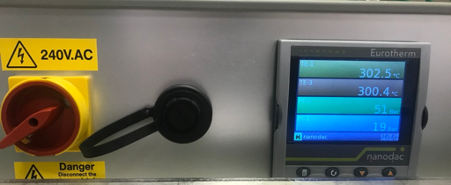
\includegraphics[width=\linewidth]{/Users/marc/Thesis/appendices/Picture1.png}
    \caption{Enrichment device control panel}
  \end{figure}

  \begin{figure}[H]
    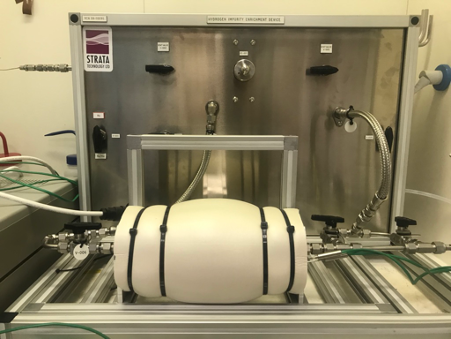
\includegraphics[width=\linewidth]{/Users/marc/Thesis/appendices/Picture2.png}
    \caption{Enrichment device chassis layout}
  \end{figure}

  \begin{figure}[H]
    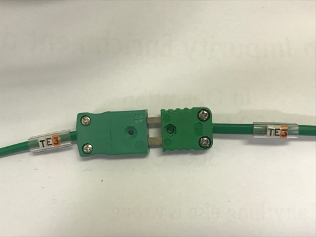
\includegraphics[width=\linewidth]{/Users/marc/Thesis/appendices/Picture3.png}
    \caption{Example of connecting thermocouples using TE3}
  \end{figure}

  \begin{figure}[H]
    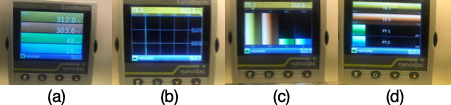
\includegraphics[width=\linewidth]{/Users/marc/Thesis/appendices/Picture4.png}
    \caption{Information based views on eurotherm control panel (a) System Summary (b) Vertical trend over time (c) Vertical bar chart (d) Horizontal bar chart}
  \end{figure}

  \begin{figure}[H]
    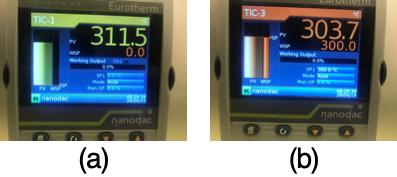
\includegraphics[width=\linewidth]{/Users/marc/Thesis/appendices/Picture5.png}
    \caption{Temperature control views}
  \end{figure}

  \begin{figure}[H]
    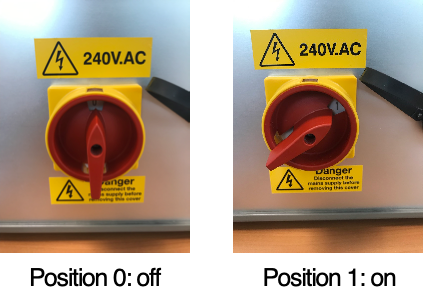
\includegraphics[width=\linewidth]{/Users/marc/Thesis/appendices/Picture6.png}
    \caption{Heating switch}
  \end{figure}

  \begin{figure}[H]
    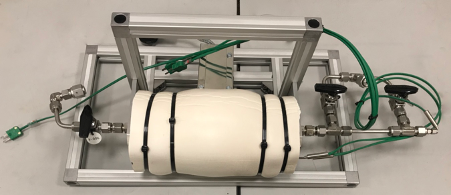
\includegraphics[width=\linewidth]{/Users/marc/Thesis/appendices/Picture7.png}
    \caption{Disconnected transportable unit}
  \end{figure}